\documentclass[palatino]{epflnotes}

\title{Mathematical modeling of DNA}
\author{Guillermo Julián Moreno}
\date{16/17 - Spring semester}

% Additional packages
\usepackage{siunitx}

% --------------------

\begin{document}
\frontmatter
\pagestyle{plain}
\maketitle

\tableofcontents
\mainmatter
% Content

\chapter{Introduction}

\section{Basics of dna}

The bases of DNA are denoted by $\mathcal{L} = \set{A,T,C,G}$ with a complementary  rule, where \begin{align*}
\conj{A} &= T &\conj{C} &= G \\
\conj{T} &= A &\conj{G} &= C
\end{align*}

An interesting? fact: the base of the DNA are antiparallel (orientation given by the orientation of the phosphate molecule).

The study of DNA can be separated in its three structures:
\begin{enumerate}
	\item The list of letters $x_i ∈ \mathcal{L} $ for $i = 1, \dotsc, 10^9$ (at least).
	\item The secondary structure is uniform: the double helix.
	\item The tertiary structure relates to the physical properties of the double helix, such as stiffness, which can vary greatly depending on the sequence (up to 25 \%), and its intrinsic shape (the shape of the central line).
\end{enumerate}

Molecular Dynamics simulations of the atoms in DNA and their surrounding medium (water) are considerably expensive, so the focus is in stochastic differential equations for which we can study output probability distribution.

The course-grained model implies simulating not all the atoms but only blocks (sugar, phosphate or whatever is a group for chemists), reducing thus the amount of degrees of freedom.

\section{Course-grained dna modeling}

We will be interested in models that predict the sequence ground-state structure and flexibility of a sequence. Each configuration space is a vector $w ∈ ℝ^N$ and the probability density function $ρ(w)$ depends on spome constants $Z,β$ and the free energy $U(w)$, so that \[ ρ(w) = \frac{1}{Z} e^{-βU(w)} \]

One special thing is four bases and not consider base pairs. ¿?

The set of parameters being modeled will by $6n$ intra-basepair and $6(n-1)$ inter-basepair degrees of freedom, so a total of $N = 12n - 6$ degrees of freedom.

For the cgDNA model, the free energy is approximated as a quadratic form \[ U(w)= \frac{1}{2} (w - μ) · K(w -μ)\] with $μ = μ(S) ∈ ℝ^N$ being the ground state configuration and $K = K(S) ∈ ℝ^{N×N}$ being the ground-state stiffness, symmetric and positive-definite.

Of course, the question is how to get those ground states $μ, K$ from the sequence $S$ you are studying. The main assumption is junction and intra-basepair interaction energies, as shown in \fref{fig:MovementsDNA}.

\begin{figure}[tbp]
\centering
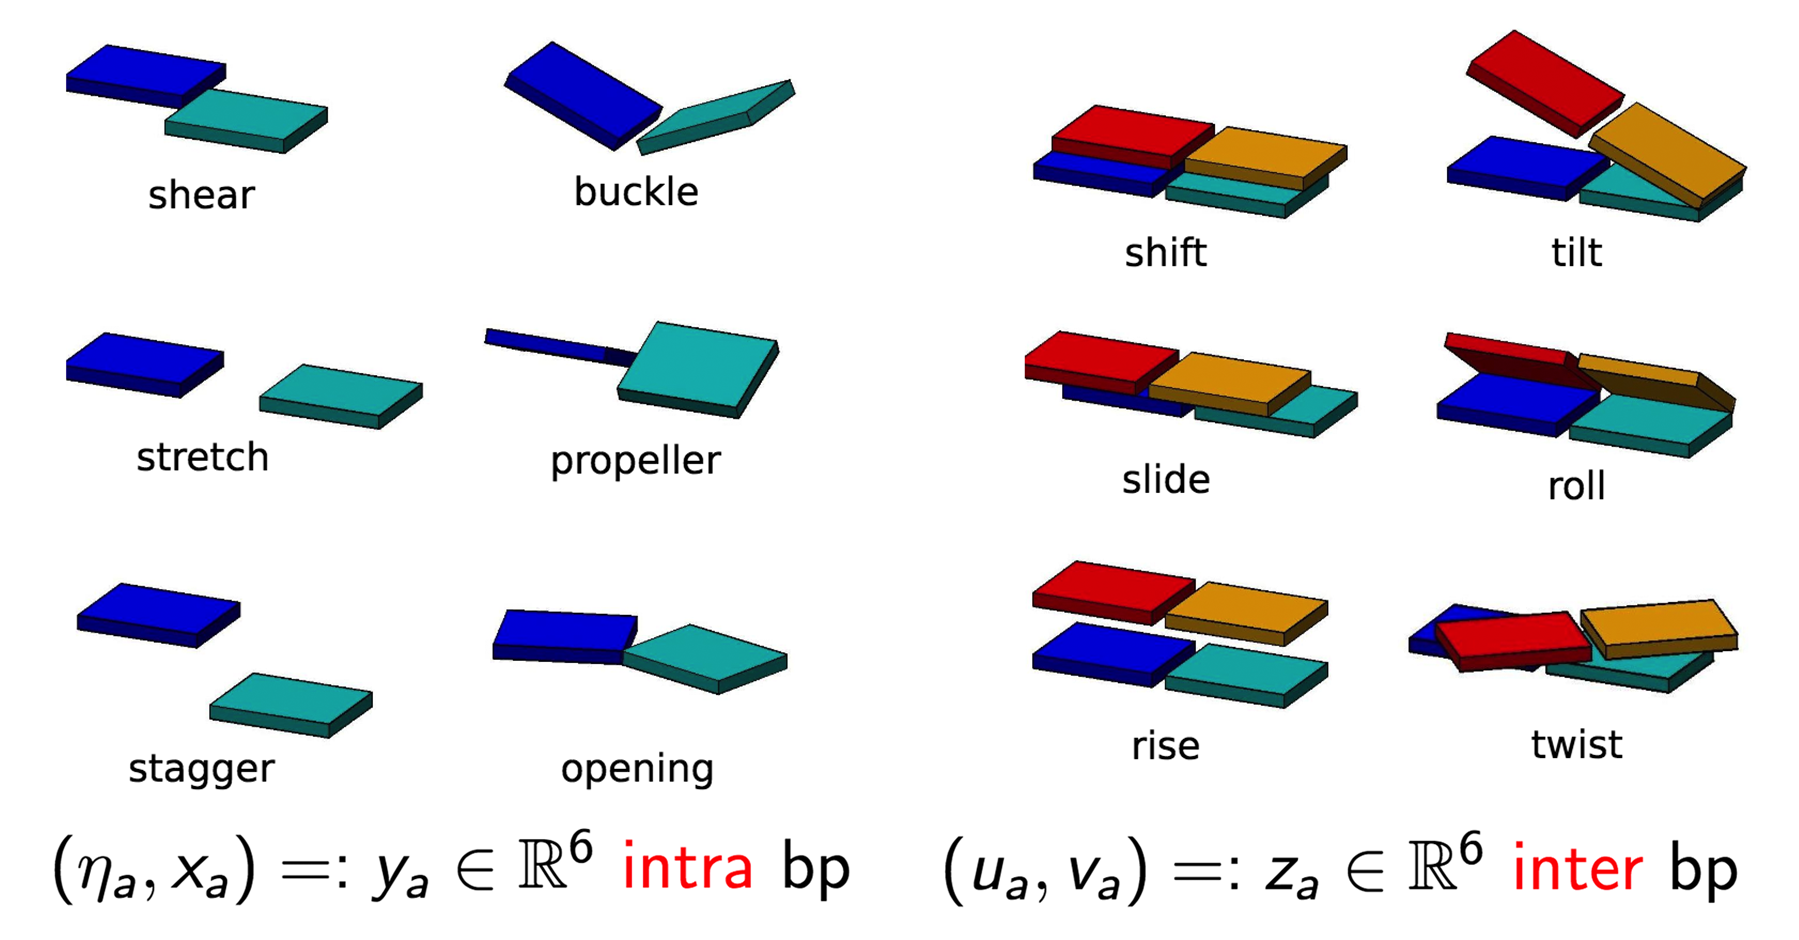
\includegraphics[width=0.8\textwidth]{img/movementsDNA.png}
\caption{Interpair and intrapair interactions}
\label{fig:MovementsDNA}
\end{figure}

\seprule[Missing week 2 and week 3 material]

I'm not sure of what I am writing but $(R_i, \vr_i)$ is the mid frame (base pair frame) between $(R_i^-, \vr_i^-)$ and $(R_i^+, \vr_i^+)$ and $\vr_i = \frac{1}{2} (\vr_i^- + \vr_i^+)$ with $R_i = R_i^-\sqrt{Q_i}$ and $Q_i = \trans{(R_i^{-})} R_i^+$ being half rotation and the relative rotation between bases.. This is a sensible notion of average in $SO(3)$. The junction frame is \[ j_i = \frac{1}{2}(\vr_i + \vr_{i+1}) \qquad i = 1, \dotsc, N\] and $J_i = R_i \sqrt{P_i}$ with $P_i = \trans{R_i} R_{i+1}$ being the relative rotation between base-pair frames.

Note: take all square root matrix multiplications on the right. We could change it to the left with no consequences\footnote{We are in $SO(3)$ so all works out. Transposes are inverses and yay.}.

We also introduce the following $4×4$ matrix representation of $SE(3)$, so that a matrix and a vector are represented by \[ \left(\begin{array}{ccc|c}
 & & &  \\
 & \mR_i& & \vec{r_i} \\
 & & &  \\ \hline
 & \vec{0} & & 1
\end{array}\right) \] and so \[ w \log \left(\begin{array}{ccc|c}
 & & &  \\
 & \mR_1 & & \vec{r_1} \\
 & & &  \\ \hline
 & \vec{0} & & 1
\end{array}\right) = \left(\begin{array}{ccc|c}
 & & &  \\
 & \mop{Id}_{3 × 3} & & \vec{0} \\
 & & &  \\ \hline
 & \vec{0} & & 1
\end{array}\right)\]

If we then know $(\mQ_i, \vq_i)$ for $i = 1,\dotsc, N$ and $(\mP_i, \vp_i)$ for $i = 1, \dotsc, N_1$ we can compute $(\mR_i^{\pm}, \vr_i^{\pm})$ or recursion \[ \begin{pmatrix} \mR_{i+1} & \vr_{i+1} \\ 0 & 1 \end{pmatrix} = \begin{pmatrix}\mR_i & \vr_i \\ 0 & 1 \end{pmatrix} \begin{pmatrix} \mP_i & \sqrt{\mP_i} \vp_i \\ 0 & 1 \end{pmatrix} \]
and at level $i$ \[ \begin{pmatrix} \mR_i^+ & \vr_i^+ \\ 0 & 1 \end{pmatrix} = \begin{pmatrix} \mR_i^{-} & \vr_i^- \\ 0 & 1 \end{pmatrix} \begin{pmatrix} \mQ_i & \sqrt{\mQ_i} \vq_i \\ 0 & 1 \end{pmatrix} \]

So it seems that what we are doing is to define the positions $(R_i, \vr_i)$ of each base pair and the positions $\pm$ of the left and right sides
.

The thing above with the $w\log$ seems to be just the initial condition with ``wlog'' beind some kind of abbreviature I don't know. It says that we eliminate overall translation and rotation of DNA so that must be it.

Then this set of equations:
\begin{gather*}
\mR_{i+1} = \mR_i \mP_i \\
\vr_{i+1} = \vr_i + \mR_i \sqrt{\mP_i} \vp_i \\
\mP_i = \trans{\mR_i}\mR_{i+1} \\
\sqrt{\mP_i} \vp_i = \trans{\mR_i} (\vr_{i+1} - \vr_{i})
\end{gather*}

So the thing is that $\vr_{i+1} - \vr_i ≝ Δ\vr_i$ is the difference between components in a fixed basis, and then writing it in the basis of the $\vr_i$ which is $\mR_{i+1}$. Here we have the weird-ass drawing of rectangles and the delta thing is the arrow.

Then coming back to $J_i = \mR_i \sqrt{\mP_i}$ and doing transposes everywhere we have that \[ \vp_i = \trans{\sqrt{\mP_i}} \trans{\mR_i} (\vr_{i+1} - \vr_{i}) = \trans{\mJ} (\vr_{i+1} - \vr_{i})\] so that $\vp_i$ is the components of $Δ\vr$ in the junction frame $\mJ$. The junction is the green thing in the drawing.

The addition of the $\sqrt{\mP_i}$ seems an unnecessary complication. But we want a simple transformation when roles of Crick and Watson strands are reversed and $\sqrt{\mP_i}$ gives a simpler transformation. That means when for some reason they want to reverse the order of the indexes, so that the $\mJ_i$ is ``like a central finite difference''.

Similarly for the base frames $\mR_i^{\pm}$, once you know the base-pair frame $(\mR_i, \vr_i)$ we have that \begin{gather*}
\mR_i^+ = \mR_i^- \mQ_i \\
(\vr_i^+ - \vr_i^-) = \mR^- \sqrt{\mQ_i}\vq_i \\
\trans{(\mR_i^-)} (\vr_i^+ - \vr_i^-) =\sqrt{\mQ_i} \vq_i
\end{gather*} where that last thing is the components of $δ\vr_i$ in the frame $\mR_i^-$. And $\vq_i$ are the components of $δ\vr_i$ in base pair frame $\mR_i$. Then more equations

\[ \mR_i^+ = \mR_i^-\mQ_i \implies \sqrt{\mQ_i} = \sqrt{\trans{(\mR_i^-)} \mR_i^+} \] and by definition we recall $\mR_i = \mR_i^- \sqrt{\mQ_i}$ this is the definition of the base-pair frame.

The introduction of the square root helps again when making crick-watson transformation rules.

This all (I suppose ``all'' from the start of the lecture?) implies a set of coordinates for a DNA configuration are the initial point $(\mR_1, \vr_1) = (\mop{Id}, \vec{0})$, the intra-pair deformation $Q_i ≝ (\mQ_i, \vq_i)$ and the inter-pair deformations $P_i ≝ (\mP_i, \vp_i)$. In turn, this allows us to work only with the $P_i, Q_i$ elements. However, $\mQ_i$ and $\mP_i$ are in $SO(3)$, that is, we have 9 entries each but there are only 3 independent entries.

So, we need to get to a minimal set of coordinates by introducing the Cayley transform. Provided that neither $\mP_i$ or $\mQ_i$ are close to rotations by π, there exists an unique mapping \begin{align*}
\appl{\cayley}{SO(3) & }{ℝ^3} \\
\mP_i &\longmapsto \vu_i \\
\mQ_i &\longmapsto \veta_i
\end{align*}

Now questions: What frame are the components of $\vu_i$? There we have in $\mR_i, \mJ_i$ or $\mR_{i+1}$?

In which frame are the components of $\veta_i$? We can have $\mR_i^-$ or $\mR_i$ or $\mR_i^+$.

A nice property of Cayley vector is that it has the same coordinates along all the frames between I don't know what because it is the axis of rotation. That applies both Cayley vectors. So it doesn't change.

Also $\mR_{i+1} = \mR_i · \cayley(\vc_i)$ where $\vc_i$ is an absolute mess of twiddles, bars and vectors with extra structure and basis and I am really tired of that.

Finally, we can explain the cgDNA model configuration coordinates. This has, for $N$ base pair ligomer a vector $\vw ∈ ℝ^{12N - 6}$ as $\vw = (\vy_1, \vz_1, \dotsc, \vz_{N-1}, \vy_N)$ where $\vz_i ∈ ℝ^6$ are the inter pair rotations and translations and $\vy_i ∈ ℝ^6$ are the intra pair rotations and translations with the rotations as a Cayley vector.

Now we worry about units. Convenient scales for translations are angstroms or nanometers, but rotations do not have dimensions. We'll see later that we need a good scaling between both for reasons yet unknown so that the units for the Cayley vector are fifths of a radian but we will see it later so then why does he mention it now.

Find names of the rotations in the PDF.

Now we omething something transformation rule. Will prove later but if $\vw$ are the coordinates for a specific configuration of the DNA fragment for one choice of the Watson strand\footnote{Define what is a strand, pls.} then the coordinates $\bar{\vw}$\footnote{In the blackboard this is $w$ with under and overbar. Such a good notation.}  are $\bar{\vw} = \mE_{2N - 1} \vw$ where \[ \mE_{2N-1} = \begin{pmatrix} 0 & \cdots & \mE \\ \vdots &\iddots & \vdots \\ \mE & \cdots & 0 \end{pmatrix} \] with $\mE ∈ ℝ^{6×6}$ just $-1, +1, +1, -1, +1, +1$ on the leading diagonal.

So the thing is the cgDNA model predicts a PDF $ρ(\vw; S, P)$ with $\vw$ the coordinates, $S$ the sequence and $P$ the parameter set. We usually suppress $S, P$ in notation. The PDF is going to work like \[ ρ(\vw) = \frac{1}{z} e^{- U(\vw)} \] where $z$ is the normalizing constant and $U$ is a quadratic polynomial in $\vw$.

We are going to do a lot of assumptions not justified and then later on we will see that they work.

So $U$ is going to look like \[ U(\vw) = \frac{1}{2} (\vw - μ(S)) \mK(S) (\vw - μ(S)) \] so we need a rule to get from $S$ to $\mK(S)$ and $μ(S)$, where $\mK(S) ∈ ℝ^{(12N - 6) × (12N - 6)}$ where $\mK(S)$ will be symmetric and positive-definite matrix. Also, $μ(S) ∈ ℝ^{12N-6}$.

We start from the formula that \[ 2U(\vw) = \sum_{i = 1}^N (\vy_i - \hat{\vy}_i) · \mK_{i}^{BP} (\vy_i - \hat{\vy}_i) + \sum_{j=1}^{N-1} (\vx_j - \hat{\vx}_j) \mK^J_j (\vx_j - \hat{\vx}_j)\] which represent respectively the sum of something over basepairs and sum over junctions, where $\vx_j = (\vy_j, \vz_i, \vy_{i+1})$. Also $\mK_i^{BP} ∈ ℝ^{6×6}$ and $\mK_{j}^J ∈ ℝ^{18 × 18}$ are symmetric.

What this means is that there is an energy term of the energy between bases in a pair which is a quadratic polynomial (assumption) with $\hat{\vy}_i$ the minimum energy position more or less. So we do a nearest-neighbor rigid base mode so now we have base to partner in base pair. Then we need to compute the energy with the other base pairs. Cross-junction interaction energies. Gross assumption that all those interaction energies are quadratic and we end with the second matrix stiffness matrix $\mK_j^J$  with $\hat{\vx}_j$ is the minimum energy configuration.

After that we do a cool linear algebra proof\footnote{That does not exist.} where we do computations\footnote{See?} where we have a vector $\vx ∈ ℝ^M$ and \[ \frac{1}{2}(\vx - \va) \mA (\vx - \va) = \frac{1}{2} ( \vx - \vb) \mB (\vx - \vb) = \frac{1}{2}( \vx - \vc) \mC (\vx - \vc)\]  with $\mA, \mB$ symmetric and positive definites. We would need a constant term (the second part is zero when $\vx = \vc$ but the first part doesn't) but this is an energy so we don't care about constants. IF you do computations then $\mC = \mA + \mB$. If you do more computations with the linear cmponents you get $\vc = \inv{\mC}(\mA \va + \mB \vb)$. We have to pad with zero because matrices are of different dimensions but everything works out. Drawings of a matrix. And in the end local sequence dependence implies non-local sequence dependence because inverses and sparses and magic.

\appendix

\chapter{Exercises}
% -*- root: ../MathModelingDNA.tex -*-

\backmatter
\printindex
\end{document}
